%Problem Set 2
%%%%%%%%%%%%%%%%%%%%%%%%%%%%%%%%%%%%%%%%%%%%%%%%

%Sweave('C:/Klaus/AAEC5126/problemsets/ps2klaus',syntax=SweaveSyntaxNoweb)

%I) DEFINE DOCUMENTCLASS AND LOAD ALL REQUIRED PACKAGES

\documentclass[11pt,reqno]{article}   %keep it simple
%\usepackage{amsmath}       % for nice math and equations
\usepackage{amsmath,amssymb}
\usepackage{graphicx}      % for fancy graphics
\usepackage{setspace}      % for basic formatting
\usepackage{enumerate}     % for more flexibility with numbered lists
  %KEY - this preserves R formatting and comments

% You may need to load all or some of these packages -
%follow the instructions on our course web site under "Help with LaTex"

%II) PREAMBLE
%%%%%%%%%%%%%%%%%%%%%%%%%%%%%%%%%%%%%%%%%%%%%%%%%%
\pagestyle{plain} %puts page number center bottom
\setlength{\topmargin}{0in}
\setlength{\textheight}{8.5in}
\setlength{\oddsidemargin}{.0in}
\setlength{\evensidemargin}{.0in}
\setlength{\textwidth}{6.5in}
\setlength{\footskip}{.5in}
\setlength{\parindent}{0in} %suppress indentation
%\onehalfspacing

\newcommand{\mlt}[1]{\mathbf{#1}} %matrix bold for Latin symbols
\newcommand{\mgr}[1]{\boldsymbol{#1}}%matrix bold for Greek symbols
\newcommand{\kR}{\tt R\rm{} }%shortcut for "R" symbol
\newcommand{\ksp}{\vspace{0.1in}}   % insert some space between chunks
%feel free to add your own shortcuts  - here a mine:
\newcommand{\kl}{\left(}
\newcommand{\kr}{\right)}
\newcommand{\kll}{\left\{}
\newcommand{\krr}{\right\}}
\newcommand{\kmu}{\mgr{\mu}}
\newcommand{\kpsi}{\mgr{\psi}}
\newcommand{\kphi}{\mgr{\phi}}
\newcommand{\kgam}{\mgr{\gamma}}
\newcommand{\ktheta}{\mgr{\theta}}
\newcommand{\kbeta}{\mgr{\beta}}
\newcommand{\kdelta}{\mgr{\delta}}
\newcommand{\kt}{^{\prime}}
\newcommand{\kdel}{\partial}
\newcommand{\kdot}{\kl . \kr}
\newcommand{\keps}{\epsilon}
\newcommand{\kkeps}{\mgr{\epsilon}}
\newcommand{\kx}{\mlt{x}}
\newcommand{\kX}{\mlt{X}}
\newcommand{\kV}{\mlt{V}}
\newcommand{\kM}{\mlt{M}}
\newcommand{\kP}{\mlt{P}}
\newcommand{\ky}{\mlt{y}}
\newcommand{\kb}{\mlt{b}}
\newcommand{\kc}{\mlt{c}}
\newcommand{\ki}{\mlt{i}}
\newcommand{\ke}{\mlt{e}}
\newcommand{\klam}{\lambda}
\newcommand{\kp}{\mlt{p}}
\newcommand{\kprob}{\text{prob}}
\newcommand{\kz}{\mlt{z}}
\newcommand{\ksig}{\sigma^2}
\newcommand{\kSig}{\mgr{\Sigma}}
\newcommand{\klog}{\text{log}}
\newcommand{\kols}{\kl \kX\kt\kX\kr^{-1}\kX\kt\ky}
\newcommand{\kSSE}{\kl \ky-\kX\kb\kr\kt\kl\ky-\kX\kb\kr}

%%%%%%%%%%%%%%%%%%%%%%%%
\usepackage{Sweave}
\begin{document}
\Sconcordance{concordance:ps2.tex:ps2.rnw:%
1 72 1 1 0 8 1 1 10 186 1 1 2 1 0 3 1 3 0 2 2 1 0 1 1 %
1 2 4 1 1 2 2 1 1 2 2 1 1 2 2 1 3 0 2 2 1 0 3 1 1 18 %
19 0 1 2 1 1 1 14 13 0 1 16 13 0 1 16 13 0 1 16 13 0 %
1 3 1 25 2 1 1 20 1 3 8 1}

%%%%%%%%%%%%%%%%%%%%%%%%

%III) TOP MATTER INFORMATION
\title{Problem Set 2}
\author{Nima Mohammadi} %ENTER YOUR NAME HERE
\maketitle %this comes at the end of the top matter to set it.



%%%%%%%%%%%%%%%%%%%%%%%%%%%%%%%%%%%%%%%%%%%%%%%%%%%%%%%%%%%%%%%%%%%%%%%%
\section*{Question 1: Orthogonality}
%%%%%%%%%%%%%%%%%%%%%%%%%%%%%%%%%%%%%%%%%%%%%%%%%%%%%%%%%%%%%%%%%%%%%%%%
Consider a CLRM with sample size $n$ and $k$ regressors.  Show that if all columns in the data matrix $\kX$
 are orthogonal to one another, the resulting solution to the Least Square problem is equivalent
 to running k separate regressions, one per explanatory variable. \\

\textit{(Hint: Partition $\kX$ into columns and express the solution formula for $\kb$ in terms of column interactions.
Then examine what this solution looks like under the stated orthogonality assumption.
Note: This is NOT asking you to do a partitioned regression.
Just a basic regression, with $\kX$ expressed in terms of its columns.) }\\

%
\begin{equation}
\begin{split} %for equations with multiple rows; each row must start with ``&''
% and end with ``\\'', except for the last one
&\kX=\begin{bmatrix} \kc_1 & \kc_2 & \ldots & \kc_k\end{bmatrix} \\
&\kX\kt = \begin{bmatrix} \kc_1\kt \\ \kc_2\kt \\ \vdots \\ \kc_k\kt\end{bmatrix} \\
& \text{Due to orthogonality columns of} \kX \text{, we have} \kc_i\kt\kc_j=0 \text{for} i\neq j\\
&\kX\kt\kX = \begin{bmatrix}
\kc_1\kt\kc_1 & 0 & \cdots & 0 \\ 
0 & \kc_2\kt\kc_2 & \cdots & 0 \\ 
\vdots & \vdots & \ddots & 0 \\ 
0 & 0 & \cdots & \kc_k\kt\kc_k \\ 
\end{bmatrix} \\
&\kl \kX\kt\kX \kr^{-1} = \begin{bmatrix}
\kc_1\kt\kc_1 & 0 & \cdots & 0 \\ 
0 & \kc_2\kt\kc_2 & \cdots & 0 \\ 
\vdots & \vdots & \ddots & 0 \\ 
0 & 0 & \cdots & \kc_k\kt\kc_k \\ 
\end{bmatrix}^{-1} =
\begin{bmatrix}
(\kc_1\kt\kc_1)^{-1} & 0 & \cdots & 0 \\ 
0 & (\kc_2\kt\kc_2)^{-1} & \cdots & 0 \\ 
\vdots & \vdots & \ddots & 0 \\ 
0 & 0 & \cdots & (\kc_k\kt\kc_k)^{-1} \\ 
\end{bmatrix} \\
\end{split}
\end{equation}
\begin{equation}
\begin{split}
& \text{Also} \\ 
& \kX\kt\ky = \begin{bmatrix} \kc_1\kt \\ \kc_2\kt \\ \vdots \\ \kc_k\kt\end{bmatrix} \ky = \begin{bmatrix} \kc_1\kt\ky \\ \kc_2\kt\ky \\ \vdots \\ \kc_k\kt\ky\end{bmatrix} \\ 
& \text{Then} \\
& \kb = \kl \kX\kt\kX \kr^{-1}\kX\kt\ky = \begin{bmatrix}
(\kc_1\kt\kc_1)^{-1} & 0 & \cdots & 0 \\ 
0 & (\kc_2\kt\kc_2)^{-1} & \cdots & 0 \\ 
\vdots & \vdots & \ddots & 0 \\ 
0 & 0 & \cdots & (\kc_k\kt\kc_k)^{-1} \\ 
\end{bmatrix} \begin{bmatrix} \kc_1\kt\ky \\ \kc_2\kt\ky \\ \vdots \\ \kc_k\kt\ky\end{bmatrix} = \begin{bmatrix} (\kc_1\kt\kc_1)^{-1}\kc_1\kt\ky \\ (\kc_2\kt\kc_2)^{-1}\kc_2\kt\ky \\ \vdots \\ (\kc_k\kt\kc_k)^{-1}\kc_k\kt\ky\end{bmatrix} = \begin{bmatrix} \kb_1 \\ \kb_2 \\ \vdots \\ \kb_k\end{bmatrix}
\end{split}
\end{equation}
In this (rather rare) occasion, the coefficients of the regression of $\ky$ on $\kX$ may be obtained via separate regressions of $\ky$ on $\kc_i$. In other words, the solution of the Least Squares problem would be equivalent to $k$ separate regressions, one for each explonatory variable. 
%%%%%%%%%%%%%%%%%%%%%%%%%%%%%%%%%%%%%%%%%%%%%%%%%%%%%%%%%%%%%%%%%%%%%%%%
\section*{Question 2: Regression on a constant}
%%%%%%%%%%%%%%%%%%%%%%%%%%%%%%%%%%%%%%%%%%%%%%%%%%%%%%%%%%%%%%%%%%%%%%%%
Consider a classical linear regression model that regresses the dependent variable, $\ky$,
against a column of ones (call it $\ki$), and no other explanatory variables.
Assume the underlying theoretical population model has the usual OLS properties.

\begin{enumerate}[(a)]
\item
Write down the underlying theoretical model for a single observation, and for the full sample of n observations.
Clearly specify the vector dimensions of each element.  Call the unknown population parameter $\mu$).

For single observation:
\begin{equation}
y_j = i_j\mu + \epsilon_j
\end{equation}
For full sample of $n$ observations:
\begin{equation}
\ky_{n\times 1} = \mlt{i}_{n\times 1}\mu + \keps_{n\times 1}
\end{equation}

\begin{itemize}
        \item $\mu$: unknown population parameter to be estimated (as $\kb$), scalar value
        \item $\ky$: dependent variable, $\left[\begin{array}{llll}{y_{1}} & {y_{2}} &{\cdots} & {y_{n}}\end{array}\right]\kt$
        \item $\mlt{i}$: independent "variable", column vector of ones
        \item $\keps$: disturbance term
\end{itemize}

\item
Derive the OLS estimator for this model (Call it $b$).
(Hint: Start with the known formula of the OLS estimator and replace the $\kX$
with the regressor for the current model.
Then simplify until you're left with a scalar that has a very well known form).

\begin{equation}
\begin{split}
& \kb = \kl \kX\kt\kX \kr^{-1}\kX\kt\ky \\
\Rightarrow & \kb = \kl \mlt{i}\kt\mlt{i} \kr^{-1}\mlt{i}\kt\ky = n^{-1}\sum^n_{j=1}y_j = \bar{y}
\end{split}
\end{equation}
The OLS estimator for this model finds the sample mean of $\ky$ as the estimation of $\mu$.
\item
Derive the variance of this estimator. Assume that the error variance $\sigma$ is known.
(Hint: Proceed as above - start with the known form of V(b), then replace the $\kX$ with
the regressor for the current model).

\begin{equation}
\begin{split}
\kV(\kb) = \sigma^2 \mathbb{E}(\kl \mlt{i}\kt\mlt{i} \kr^{-1}) = \frac{\sigma^2}{n}
\end{split}
\end{equation}

\item
Show that the OLS estimator for your model is unbiased for the underlying population parameter.

\begin{equation}
\begin{split}
\mathbb{E}(\kb) & = \mathbb{E}(\bar{y}) = \mathbb{E}(\frac{1}{n}\sum^n_{j=1}y_j) = \frac{1}{n}\mathbb{E}(\sum^n_{j=1}y_j) \\ & = \frac{1}{n}\sum^n_{j=1}\mathbb{E}(y_j) = \frac{1}{n}\sum^n_{j=1}\mu = \frac{1}{n}n\mu = \mu
\end{split}
\end{equation}

\item
In light of your results, can you make a general statement regarding the best linear unbiased
 estimator for the population mean when no explanatory variables are available?
 
 In part (b) we saw that in absence of explanatory variables, the OLS estimator is equal to the sample mean $\bar{y}$. The Gauss-Markov theorem shows that this estimator of population mean is 'BLUE'. Part (d) showed us the unbiasedness of this estimator whereas in part (d) the consistency of the model is shown. Comparing the variance with thereof other estimators indicates the relative efficiency of the OLS estimator. In conclusion, the OLS estimator of poulation mean gives the lowest variance of the estimate, as compared to other unbiased, linear estimators.
\end{enumerate}

%%%%%%%%%%%%%%%%%%%%%%%%%%%%%%%%%%%%%%%%%%%%%%%%%%%%%%%%%%%%%%%%%%%%%%%%
\section*{Question 3: Small Sample Properties of a
Linear regression Model with non-zero-mean-error}
%%%%%%%%%%%%%%%%%%%%%%%%%%%%%%%%%%%%%%%%%%%%%%%%%%%%%%%%%%%%%%%%%%%%%%%%
Consider the TRUE linear regression model $\ky=\ki\beta_1 + \kX\kbeta_2+\kkeps$
 where $\ki$ is an n by 1 column of 1's, and $\kX$ is an n by (k-1) matrix of regressors.
 Assume that the n elements of the random error vector $\kkeps$ are distributed
 i.i.d normal with variance $\sigma^2$, but with mean $\mu \neq 0$. As usual,
 assume that the elements in $\kkeps$ are uncorrelated with the elements in $\kX$.

\begin{enumerate}
\item
Because the mean of $\epsilon$ is not zero, hence assumptions 3 and assumption 5 are violated by this specification. 
\item
We want to show that via Partitioned Regression, the estimator of the coefficient parameters for this model will produce unbiased slope estimation, but that the estimation for the intercept will be biased. We will indicate the estimated intercept as $b_1$ and the vector of remaining estimated parameters as $b_2$ with true parameter values $\beta_1$ and $\beta_2$, respectively. The functional form for the partitioned regression will be $y = X_1\beta_1 + X_2\beta_2$, where $X_1$ is a vector of ones. Then the estimator of $\beta_2$ will be $b_2 = (X_2\kt M_1 X_2)^{-1}X_2\kt M_1y$
where $\mlt{M}_1=\mlt{I}-i(i\kt i)^{-1}i\kt$ represents the deviation-from-the-mean matrix.

\begin{equation}
\begin{split}
\mathrm{b}_{2}&=\left(X_{2}^{\prime} M_{1} X_{2}^{\prime}\right)^{-1} X_{2}^{\prime} M_{1}\left(X_{1} \beta_{1}+X_{2} \beta_{2}+\epsilon\right)\\
&=\left(X_{2}^{\prime} M_{1} X_{2}\right)^{-1} X_{2}^{\prime} M_{1} X_{1} \beta_{1}+\left(X_{2}^{\prime} M_{1} X_{2}\right)^{-1} X_{2}^{\prime} M_{1} X_{2} \beta_{2}+\left(X_{2}^{\prime} M_{1} X_{2}\right)^{-1} X_{2}^{\prime} M_{1} \epsilon\\
M_{2}&=I-X_{2}\left(X_{2}^{\prime} X_{2}\right)^{-1} X_{2}^{\prime} \rightarrow M_{2}X_{2} = 0\\
\text{and}\\
M_{1}&=I-X_{1}\left(X_{1}^{\prime} X_{1}\right)^{-1} X_{1}^{\prime} \rightarrow M_{1} X_{1}=0\\
&\mathbf{b}_{2}=\left(X_{2}^{\prime} M_{1} X_{2}\right)^{-1} X_{2}^{\prime} M_{1} X_{2} \beta_{2}+\left(X_{2}^{\prime} M_{1} X_{2}\right)^{-1} X_{2}^{\prime} M_{1}\epsilon\\
& \text{Also we have } M_{1} \epsilon=\epsilon-i \bar{\epsilon}=\epsilon-i \mu \longrightarrow E_{\epsilon}\left(\mathbf{b}_{2} | X\right)=\beta_{2}+\left(\left(X_{2}^{\prime} M_{1} X_{2}\right)^{-1} X_{2}^{\prime} E_{\epsilon}(\epsilon-i \mu) | X)\right.\\
&\left.E_{\epsilon}((\epsilon-i \mu)| X\right)=i \mu-i \mu=0 \longrightarrow E\left(b_{2}\right)=\beta_2 \longrightarrow \text{Then } b_2 \text{ is an unbiased estimator for the real} \beta_2.
\end{split}
\end{equation}

For $b_1$ we have $b_{1}=\left(X_{A}^{\prime} M_{2} X_{1}\right)^{-1} X_{1}^{\prime} M_{2} y=\left(X_{1}^{\prime} M_{2} X_{1}\right)^{-1} X_{1}^{\prime} M_{2}\left(X_{1} \beta_{1}+X_{2} \beta_{2}+\epsilon\right)$

Since we have $M_2X_2=0$:
$$E\left(b_{1}\right)=\beta_{1}+E\left[\left(X_{1}^{\prime} M_{2} X_{1}\right)^{-1} X_{1}^{\prime} M_{2} \epsilon\right]=\beta_{1}+\left(X_{1}^{\prime} M_{2} X_{1}\right)^{-1} X_{1}^{\prime} E\left(M_{2} \epsilon\right) = \beta_1+\mu$$
Since the expected value of $M_2\epsilon$ is not zero in this case, expected value of $b_1$ is not equal to $\beta_1$, so it is a biased estimator.


\item
Now we assume the true model is as before, but the analyst chooses to estimate it without an intercept. Continuing to assume the above given properties of the error term, we want to show that in this case the OLS estimator $\mathbf{b}_{2}$ will be biased.

\begin{equation}
\begin{split}
&b=\left(X^{\prime} X\right)^{-1} X^{\prime} y=\left(X^{\prime} X\right)^{-1} X^{\prime}(X \beta+\epsilon)=\beta+\left(X^{\prime} X\right)^{-1} X^{\prime} \epsilon\\
&\Rightarrow E_{\epsilon}(b | X)=E_{\epsilon}\left(\left(\beta+\left(X^{\prime} X\right)^{-1} X^{\prime} \epsilon\right) | X\right)\\&=\beta+\left(X^{\prime} X\right)^{-1} X^{\prime} E_{\epsilon}(\epsilon | X)= 
\beta+\left(X^{\prime} X\right)^{-1} X^{\prime} \mu\\
&\left.\Rightarrow E(b)=E_{X}\left(E_{\epsilon}\langle b| X\right)\right)=E_{X}(\beta)+E_{X}\left(\left(X^{\prime} X\right)^{-1} X^{\prime} \mu\right)= \beta+(X\kt X)^{-1}X\kt\mu \neq \beta
\end{split}
\end{equation}
So the estimator is biased.
\item 
The reason for biasedness of $b$ in the previous part is that we do not have an intercept in our model preventing us from capturing the effects of a non-zero mean error term in the intercept. But, in part 2 we could split the model and the effects of the non-zero mean would be capture by $b_1$ and therefore $b_2$ is an unbiased estimator, but now in this setting we do not have intercept and the whole $b$ as the estimator of beta matrix is consequently biased. 

\end{enumerate}


%%%%%%%%%%%%%%%%%%%%%%%%%%%%%%%%%%%%%%%%%%%%%%%%%%%%%%%%%%%%%%%%%%%%%%%%
\section*{Question 4: Variance of OLS estimator}
%%%%%%%%%%%%%%%%%%%%%%%%%%%%%%%%%%%%%%%%%%%%%%%%%%%%%%%%%%%%%%%%%%%%%%%%
Consider script \texttt{mod1s3}, which deals with the small sample properties of the OLS estimator.

In this exercise you will show that the empirical standard deviations ("standard errors") of the OLS estimator
depend on the variability in $\kX$. Specifically, perform the following simulation tasks
(make sure all your tables and figures are labeled clearly and correctly):

\begin{Schunk}
\begin{Sinput}
R> set.seed(37)
R> N <- 1000 #population size
R> n <- 1000 #sample size
R> r1 <- 500 #number of error vectors to draw
\end{Sinput}
\end{Schunk}

\begin{Schunk}
\begin{Sinput}
R> bvec<-c(1, .5, 1.2)
R> sig <- 1
R> x1 <- rep(1, N)
R> x2 <- rnorm(N, 3, 1)
R> x3 <- rnorm(N, -2, 1)
R> X1 <- cbind(x1, x2, x3)
R> k <- ncol(X1)
R> x2 <- rnorm(N, 3, 3)
R> x3 <- rnorm(N, -2, 3)
R> X2 <- cbind(x1, x2, x3)
R> x2 <- rnorm(N, 3, 4)
R> x3 <- rnorm(N, -2, 4)
R> X3 <- cbind(x1, x2, x3)
R> x2 <- rnorm(N, 3, 6)
R> x3 <- rnorm(N, -2, 6)
R> X4 <- cbind(x1, x2, x3)
\end{Sinput}
\end{Schunk}

\begin{Schunk}
\begin{Sinput}
R> bmat1 <- matrix(0, k, r1)
R> bmat2 <- matrix(0, k, r1)
R> bmat3 <- matrix(0, k, r1)
R> bmat4 <- matrix(0, k, r1)
R> for (i in 1:r1){
         eps <- rnorm(n, 0, sig)
         y1 <- X1 %*% bvec + eps
         y2 <- X2 %*% bvec + eps
         y3 <- X3 %*% bvec + eps
         y4 <- X4 %*% bvec + eps
         
         b1 <- solve((t(X1)) %*% X1) %*% (t(X1) %*% y1)
         b2 <- solve((t(X2)) %*% X2) %*% (t(X2) %*% y2)
         b3 <- solve((t(X3)) %*% X3) %*% (t(X3) %*% y3)
         b4 <- solve((t(X4)) %*% X4) %*% (t(X4) %*% y4)
         
         bmat1[, i] <- b1
         bmat2[, i] <- b2
         bmat3[, i] <- b3
         bmat4[, i] <- b4
 }
\end{Sinput}
\end{Schunk}


% latex table generated in R 3.6.2 by xtable 1.8-4 package
% Thu Feb 27 08:57:32 2020
\begin{table}[!h]
\centering
\caption{Sampling distribution, std(x2)=std(x3)=1} 
\begin{tabular}{lrrr}
  \hline
variable & true value & mean (samp.dist.) & std (samp.dist) \\ 
  \hline
constant & 1.0000 & 0.9939 & 0.1138 \\ 
  x2 & 0.5000 & 0.5018 & 0.0316 \\ 
  x3 & 1.2000 & 1.2002 & 0.0306 \\ 
   \hline
\end{tabular}
\end{table}% latex table generated in R 3.6.2 by xtable 1.8-4 package
% Thu Feb 27 08:57:32 2020
\begin{table}[!h]
\centering
\caption{Sampling distribution, std(x2)=std(x3)=3} 
\begin{tabular}{lrrr}
  \hline
variable & true value & mean (samp.dist.) & std (samp.dist) \\ 
  \hline
constant & 1.0000 & 1.0001 & 0.0484 \\ 
  x2 & 0.5000 & 0.4999 & 0.0110 \\ 
  x3 & 1.2000 & 1.2005 & 0.0098 \\ 
   \hline
\end{tabular}
\end{table}% latex table generated in R 3.6.2 by xtable 1.8-4 package
% Thu Feb 27 08:57:32 2020
\begin{table}[!h]
\centering
\caption{Sampling distribution, std(x2)=std(x3)=4} 
\begin{tabular}{lrrr}
  \hline
variable & true value & mean (samp.dist.) & std (samp.dist) \\ 
  \hline
constant & 1.0000 & 1.0019 & 0.0412 \\ 
  x2 & 0.5000 & 0.4991 & 0.0081 \\ 
  x3 & 1.2000 & 1.2002 & 0.0076 \\ 
   \hline
\end{tabular}
\end{table}% latex table generated in R 3.6.2 by xtable 1.8-4 package
% Thu Feb 27 08:57:32 2020
\begin{table}[!h]
\centering
\caption{Sampling distribution, std(x2)=std(x3)=6} 
\begin{tabular}{lrrr}
  \hline
variable & true value & mean (samp.dist.) & std (samp.dist) \\ 
  \hline
constant & 1.0000 & 1.0019 & 0.0349 \\ 
  x2 & 0.5000 & 0.4991 & 0.0055 \\ 
  x3 & 1.2000 & 1.2002 & 0.0052 \\ 
   \hline
\end{tabular}
\end{table}

\begin{figure}[!ht]
\centering
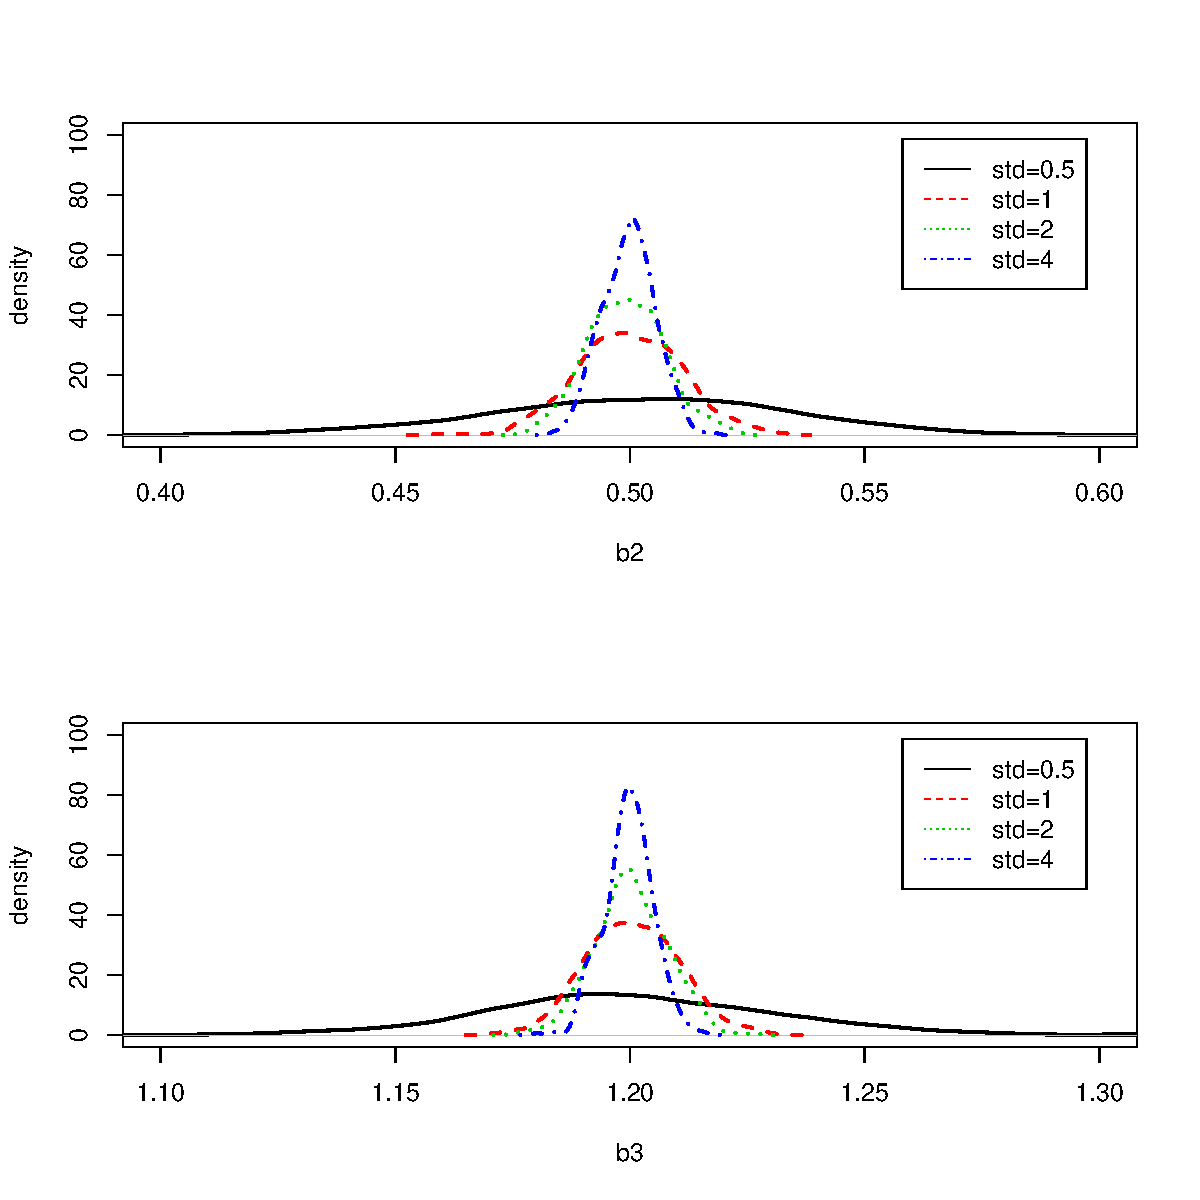
\includegraphics{ps2-R7}
\caption{CONDITIONAL Sampling distribution for OLS estimates at different settings for the coefficients of x2 and x3}
\label{fig:combos}
\end{figure}

As implied by $Var(\kb) = \sigma^2(\kX\kt\kX)^{-1}$, with increase of the variance of covariates $\kX$ we will have decrease of variance for $\kb$. Interestingly there is an inverse relation between the variance of the explonatory variables and the standard deviation of parameter estimations. This suggests that with higher explanatory power the distribution of of estimated values become narrower. Consequently, we will have more significant estimations and observe increase in t-value. The figures and tables above confirm our findings. 


\end{document}        

